\subsection{Simulation Efficiency}
\paragraph{}
It is also worth noting that the method that I am using to simulate the orbits is generally known as being a brute force method, where every body in the simulation has all of its forces simulated based on every other body in the simulation, while this enables the most accurate method of simulation, it is not particularly efficient, and only really works well for small numbers of bodies, meaning that it would suit the purposes of this program.

\paragraph{}
There are some forces that will be calculated to be so insignificant that it will not majorly affect the outcome of the simulation. For example, the orbit of two bodies will not be massively affected by a third body that is extremely far away. 

\paragraph{}
This principle is applied in the Barnes-Hut Algorithm, in which space is divided up into a quadtree. (octree for 3D simulation.) In this method, only particles/bodies that are close to the particle being simulated will be individually simulated. Particles that are further away will be simulated as one large particle based on its center of mass. This mainly increases the effectiveness if there are a large number of particles in a particular area, as this greatly reduces the number of interactions that need to be calculated.

\paragraph{}
While this method would have some benefits, the method is mainly designed for simulations with thousands of bodies or particles, something that is outside the scope for this project, it also makes use of a relatively complex algorithm that could be difficult to replicate in the time that I have available.

\paragraph{}
This may be something that is worth investigating at a later date should there be time, particularly if there is a need to simulate multiple thousands of bodies.

\paragraph{}
It may be possible to save some computational time by computing the values force forces inside a matrix. This would describe every particle to particle permutation that is possible and thus the forces between them in a undirected, weighted graph. While it won't really be used as a graph, it is a valid abstraction for the computation, removing duplication of a calculation that would decrease calculation performance.

\subsection{Simulation Prototyping}
\begin{wrapfigure}{r}{0.5\textwidth}
  \centering
  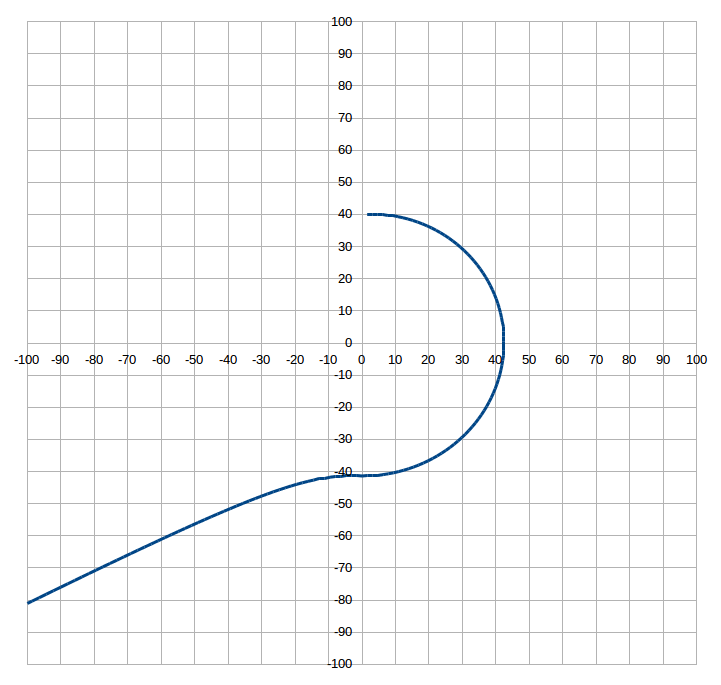
\includegraphics[width=0.45\textwidth]{img/notworking0.png}
  \caption{Inverted Negative Quadrant}
  \vspace{-10pt}
\end{wrapfigure}

\paragraph{}
The main thing that I wanted to check in the design of the project is that the mechanics that I plan to use will work correctly and as intended, due to the sheer volume of data involved, the easiest way to deal with this is to write a small program that runs through a simple scenario.

\paragraph{}
I started by writing a program that ran through a two body problem, using the intended algorithm and a fixed one second time step, I adjusted the gravitational constant to a more manageable number (1) that would work for small values of mass and velocity. 

\paragraph{}
After the program was running, I set up a quick terminal output of the position of the body, these values were then pasted directly into a spreadsheet application and displayed on a graph, much to my dismay, it did not quite work correctly, the expected result of this should be a near perfect circle that loops back on itself, the system is theoretically closed and should remain constant.

\paragraph{}
However this output clearly shows that the object completes half an orbit, and then suddenly decides to veer off in completely the wrong direction, this results in the distance to the body becoming greater and the force diminishing.

\paragraph{}
When looking at the other values, particularly the angle of the orbiting body to the barycentre (0, 0, fixed mass), the angle flips its sign, from ~-1.5 Radians to ~1.5 Radians, this causes the forces to also flip their sign and the forces then act in the opposite direction, causing acceleration away from the central body into infinity.

\paragraph{}
The fix for this was to check when the orbit crosses the X axis and flip the sign of the resultant forces when it does so that the system remains in orbit, this works in preventing this problem, however it manages to highlight a new issue.

\begin{wrapfigure}{!hl}{0.5\textwidth}
  \centering
  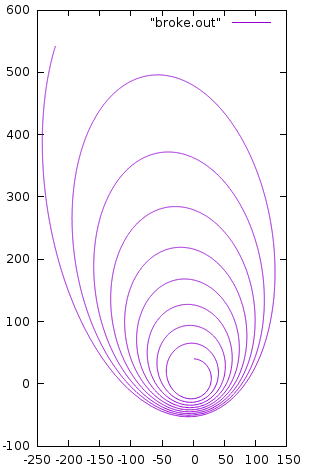
\includegraphics[width=0.45\textwidth]{img/notworking1amp.png}
  \caption{Extreme KE Increase}
  \vspace{-10pt}
\end{wrapfigure}

\paragraph{}
As the body orbits, its height increases dramatically, and mainly on the negative X side of the graph, it is pretty clear that energy is not being conserved in this closed system and the orbiting body is gaining energy allowing it to reach a higher and higher orbit.

\paragraph{}
Upon further reading, it appears that this is simply a flaw of the system that I have elected to use, known generally as Euler's Method, while this method is relatively simple to implement, it comes with significant disadvantages, the main one being is that a much smaller time base is required when bodies become extremely close together, meaning that a fixed time base will not be an option. The method does not maintain conservation of energy and orbits will become higher over time due to error accumulated in the equations, the sheer amount of calculations that need to be done only worsen this effect, this is more obvious when looking at a highly eccentric orbit. while I understood that this would be the case, I did not consider that it would be quite this severe.

\begin{wrapfigure}{r}{0.45\textwidth}
  \centering
  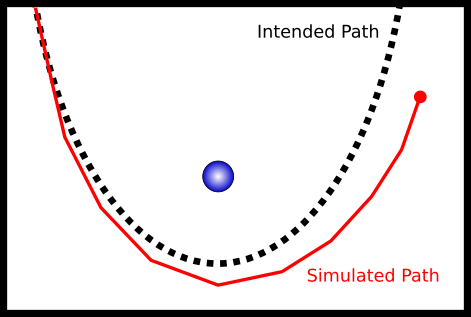
\includegraphics[width=0.4\textwidth]{img/orbitbad.png}
  \caption{Integration Deviation}
  \vspace{-10pt}
\end{wrapfigure}

\paragraph{}
At a mathematical level, the algorithm is performing a method of numerical integration through the equation $s=ut+\frac{1}{2}at^2$ which in essence will find the area under a velocity / time graph which equates to the distance travelled. This method performs this equation at every single time step, during the time the acceleration is constant and it is performed over the provided time step. This results in an issue when the orbiting body is close to the central body, as the distance travelled over the fixed time step becomes too large to correctly map to the intended orbit path, which causes the accumulation of error and instability over time. This is widely known as Euler Integration, Acceleration, Velocity and Position ($a \rightarrow v \rightarrow r$) are all updated sequentially in each time step.

\subsubsection{Leapfrog Intergration}
\paragraph{}
After some research into this problem, it was clear that this is not a problem that can be solved while still retaining the simple sequential $a \rightarrow v \rightarrow r$ calculation flow and would require some investigation into alternate methods. One of the numerical integration methods that is commonly used in gravitational particle simulations is Leapfrog integration, this method involves updating the velocity half time step out of phase with the acceleration and position, hence the name leapfrog.

\begin{figure}[!ht]
  \centering
  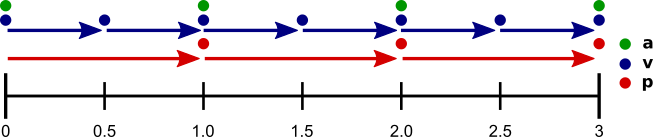
\includegraphics[width=0.6\textwidth]{img/leapfrog.png}
  \caption{Leapfrog Flow}
\end{figure}

\paragraph{}
Because it is somewhat difficult to step for half an iteration as integer loop counters are generally preferred for performance reasons, there are versions of these equations that are synchronised to update simultaneously. This effectively then becomes a calculation flow of $\frac{1}{2}v \rightarrow r \rightarrow a \rightarrow \frac{1}{2}v$.

\begin{figure}[!ht]
  $$x_{i+1}=x_i+v_i\Delta{t}+\frac{1}{2}a_i\Delta{t}^2$$
  $$v_{i+1}=v_i+\frac{1}{2}(a_i+a_{i+1})\Delta{t}$$
  \caption{Time-step Synchronised Leapfrog Formula}
\end{figure}

\subsubsection{Vector Equations}
\paragraph{}
These equations will apply to the the components of the vectors, the acceleration of the body is calculated using the universal gravitation calculation and the resulting force can be divided by the mass of the body in order to get the acceleration. This can then be broken into x and y components and calculations can be performed on individual axis. The issue with this is that this requires the use of trigonometric functions both to find angles and to work out the ratios for components, these can come a quite high computational cost, while in low volumes this should not be an issue, with a larger number of bodies it could cause significant slow down.

\paragraph{}
Another issue that these functions can cause is when it comes to moving through a coordinate system, when an object goes negative on the x axis the sign on the angle becomes negative which results in the forces flipping, while this can be corrected it is somewhat messy and could cause issues further down the line.

\paragraph{}
A better way to compute the components is to directly calculate the forces as components by using a vector equation on both axis, this means that the trigonometric functions will not be necessary for the main simulation loop of the program, greatly improving the performance of said simulation.\\\

In this form the equation for force becomes:

$$F_{xy}=\frac{Gm_1m_2}{r^3} \cdot \hat{r_{xy}}$$

The proof for this formula can be found in the document appendix.

\paragraph{}
The benefit of using this equation over the trigonometric equation is found in small benefits to performance, when it comes to the large amount of calculations that are required per second, but also when it comes to the complexity of the code, resulting in a program that is far easier to maintain and understand in the long run.

\paragraph{}
There will still be some cases where the trigonometric functions are required, for example it may be necessary when setting up bodies and the direction of their initial velocity, as it would be more understandable to the user to define starting conditions in terms of angle and magnitude.